\documentclass[a4paper,10pt]{apuntes}
\usepackage{anysize} 
\usepackage{dsfont}
\usepackage{amssymb}
\usepackage{textcomp}
\usepackage{plain}
\marginsize{3cm}{2cm}{2cm}{2cm} 

%opening
\title{Estructuras algebraicas}
\author{Pedro Valero Mejía \\ Guillermo Ruiz Álvarez}
\date{2013 / 2014}

\newenvironment{notacion}[1][Notación:]{\begin{trivlist}
\item[\hskip \labelsep {\bfseries #1}]}{\end{trivlist}}

\begin{document}

\maketitle
\tableofcontents
\newpage

\section{Grupos}
 
 Por definición, sea X un conjunto no vacío, podemos construir el conjunto de pares ordenados $X\ast X=\{(x,y)/x,y\in X\}$\\
 Vamos a fijar un conjunto $X\neq \varnothing$  y una función $\appl{\varphi}{X\ast X}{X}$ que a cada par $(x,y)$ le asocia un elemento $\varphi (x,y) \in X$ que expresamos como $x\ast y$, siendo $\ast$ cualquier operación.
 
 \begin{defn}[Conjunto\IS cerrado por la operación]
  Sea $S$ un subconjunto no vacío de $G$, diremos que $S$ es cerrado por $\varphi$  si la combinación por $\varphi$  de dos elementos de S da otro elemento del mismo conjunto.
 \end{defn}
 
 Dados $x,y,z \in X$ puede ser interesante el resultado $x\ast y\ast z$ pero, por definición, esto no tiene sentido. Sin embargo, si tendrían 
 sentido $(x\ast y)\ast z$ ó $x\ast (y\ast z)$. Estas operaciones podrían tener, o no, el mismo resultado. Queremos un conjunto con una operación 
 donde no tengamos que preocuparnos por la colocación de los paréntesis. Para ello debemos buscar una operación asociativa.
 
 \begin{defn}[Grupo]
 Dado $G\neq \varnothing$  y $\varphi: G*G \longrightarrow$  $G$, diremos que $G$ es un grupo si:
 \begin{enumerate}
  \item La operación de {$(G,*)$ es asociativa.}
  \item Existencia del neutro: {$\exists e \in G \tq \forall x\in G: x\ast e=e\ast x=x$}
  \item Existencia del inverso: {$\forall x \in G\  \exists  x'  \in G \tq x*x'=x'*x=e$}
 \end{enumerate}
 \end{defn}

 \begin{example}
   $(\mathbb{Z}, +);\ (\mathbb{R}, +);\ (\mathbb{R}-\{ 0\} , \cdot);\ (\mathbb{R}/x>0, \cdot)$ son grupos, mientras que 
  $(\mathbb{Z}, \cdot);\ (\mathbb{R}, \cdot)$ no lo son.
   
   A partir de un conjunto $A$ definimos $B(A)$ como el conjunto de todas las biyecciones de $A$ en sí mismo. Puesto que la composicón 
   de dos biyecciones es otra biyección, la composición es una operación definida sobre $B(A)$. Si tomamos como elemento $e$ la biyección 
   identidad y como $x'$ la función inversa, podemos comprobar que $B(A)$ es un grupo respecto a la composición.
 \end{example}
  
\begin{theorem}
	En todo grupo se cumplen las propiedades de unicidad del elemento neutro y del inverso.  
\end{theorem} 

 \begin{proof}
 \\Sean $e$, y $e'$ dos elementos neutros de nuestro grupo $G$, se cumple que $e*e'=e'$, pero tambien se cumple que $e'*e=e$. Esto implica que $e'=e$.

 Por otro lado, si suponemos la existencia de dos elementos inversos $a',a''\in G$, entonces $e=a*a'=a*a''$. Si operamos con $a'$ en ambos lados de la ecuación tenemos: $a'*(a*a')=a*(a'*a'')$, pudiendo reordenar los paréntesis por la propiedad asociativa. Así pues, obtenemos $a'=a''$.
 En esta última demostración nos hemos apoyado en la propiedad cancelativa, que sólo se presenta cuando trabajamos en un grupo.
 \end{proof}
 
 \begin{defn}[Propiedad\IS cancelativa]
 Si $a,b,c\in G$ siendo $G$ un grupo tenemos que $$b\ast a = c\ast a \implies b = c$$ $$a\ast b = a\ast c \implies b = c$$
 \end{defn}
  
 \begin{defn}[Transformación\IS lineal rígida]
  Son aquellas que conservan las distancias. (En $\mathbb{R}^{2}$  sólo están las simetrías y giros).
 \end{defn}
 
 \begin{example} 
  Vamos a trabajar con un triángulo equilátero, $\Delta$  en $\mathbb{R}^{2}$  y vamos a encontrar el conjunto de todas las aplicaciones lineales rígidas 
  que llevan el triángulo en si mismo. $D_{3}=\{f\in G / f(\Delta)\longrightarrow\Delta\}$.\\
  Para empezar, dentro de este grupo encontramos todos los giros de águlo 120º. Si defino $a=g_{2\pi/3}$, tenemos las aplicaciones:
  $e$, $a$  y $a*a$, ya que la aplicación $a*a*a=e$, $a*a*a*a=a$  y así sucesivamente, por completar vueltas al círculo unidad.\\
  Por otro lado, también tenemos las simetrías que tienen como eje las alturas del triángulo. Denotaremos estas simetrías como: $S_{1}$, $S_{2}$  y $S_{3}$.
  Sabemos que la combinación de un giro y una simetría tiene como resultado otra simetría. Si combinamos $a*S_{1}$  obtenemos otra simetría, 
  que también deja el triángulo en si mismo. Así pues, esta simetría, debe tratarse de $S_{2}$  ó $S_{3}$. Lo mismo ocurre con $a*a*S_{1}$.
  
  Así, tenemos: $D_{3}=\{e, a, a*a, S_{1}, a*S_{1}, a^{2}*S_{1}\}$
 \end{example}

 La representación geométrica de un grupo consiste en la descripción de los elementos geométricos que lo constituyen. En el 
 caso del ejemplo, consistiría en indicar qué giros y simetrías constituyen el grupo.
 La representación abstracta o algebraica de un grupo suele realizarse por medio de una tabla, o una serie de restricciones sobre las operaciones
 de combinación de los elementos del grupo, sin necesidad de indicar qué es realmente cada elemento.
 \begin{example}
  La representación abstracta de $D_{3}$  viene dada por tres condiciones:
 \begin{itemize}
  \item ord(g)=3
  \item ord(s)=2
  \item $g*s=s*g^{2}$
 \end{itemize}
 Ya que con estas condiciones podríamos construir una tabla con todas las combinaciones 2 a 2 de elementos del grupo sin necesidad
 de saber nada acerca de esos elementos.
 \end{example}
 
 \begin{defn}[Orden\IS finito]
  Se dice que un elemento $a\in G$, siendo G un grupo, tiene orden finito si $\exists k\in\mathbb{N} \tq  a^{k}=e$.
 \end{defn}
 
 \begin{defn}[Orden\IS de un elemento]
  Dado un elemento de orden finitio, decimos que su orden es el menor entero positivo con el que se cumple $a^{k}=e$.
 \end{defn}
 
 \begin{defn}[Orden\IS de un grupo]
 El orden de un grupo es el número de elementos del mismo, esto es, su cardinalidad.
 \end{defn}
 
\subsection{Subgrupos}
 Sea $G$ un conjunto y $\varphi$  la operación con la que forma un grupo, vamos a ver cuando un subconjunto de G es un grupo de forma natural,
 esto es lo que denominaremos subgrupo.
 
 \begin{defn}[Subgrupo]
  Diremos que un subconjunto no vacío $S$ de un grupo $H$ es un subgrupo de $H$ (notación: $S < H$) si:
  \begin{enumerate}
   \item $S$ es cerrado por la operación.
   \item $e \in S$.
   \item $s \in S \implies s^{-1}\in S$.
  \end{enumerate}
  
  Es decir, si $S$ es un grupo y es a su vez subconjunto de $H$, entonces $S$ es subgrupo.
 \end{defn}
 
  \begin{theorem}
   Dado un conjunto numerable de subgrupos $\{ S_i \}$, entonces $\bigcap S_i $ es un subgrupo.
  \end{theorem}

  
  \begin{defn}[Grupo\IS generado por un elemento]
   Fijado un elemento g $\in$G, definimos el grupo generado por g como:\\
   $<g>$=$\{$..., $g^{-2}$, $g^{-1}$, e, g, $g^{2}$,...$\}$. Este grupo es un subgrupo de G
  \end{defn}

  \begin{theorem}
   Si H es un subgrupo de G y $g\in H$ entonces $\gen{g} \subset H$.   
  \end{theorem}

  A partir de un conjunto $C=\{g_{1}$, $g_{2}$, $g_{3}$... $g_{s}\}$, contenido en $G$, vamos a buscar el menor subgrupo que lo contiene.
  $<g_{1}$, $g_{2}$, $g_{3}$... $g_{s}>$=$\displaystyle \cup_{k\in\mathbb{N}}$  $\{ a_{1}\ast a_{2}\ast a_{3}\ast \hdots \ast a_{k} \tq (a_{i}\in C) \vee ( a_{i}\in C^{-1} ) \}$. Es un subgrupo que contiene a 
  todos los elementos de C.
  
  Si H es un subgrupo que contiene a los elementos de C, el grupo generado por esos elementos se contiene en H.
  
  \begin{defn}[Grupo\IS cíclico]
   Dado $H<G$ se dice que $H$ es cícilico si existe $g\in G\tq \{ H=<g>\} $. 
  \end{defn}

  \begin{theorem}
   Si G es un grupo finito y $S \subset G$ es un subconjunto no vacío $\implies$ \\S es un subgrupo $\iff$ S es cerrado por la operación.   
  \end{theorem}
  
  \begin{proof}
   La implicación hacia la derecha es obvia por la propia definición de subgrupo.
   Para la implicación hacia la izquierda partimos de que S es cerrado y finito. Por tanto $\exists d \in S \tq ord(d)=n$ y $<d>\ \subset S$
   $\implies$ $d^{n}=e\in S$ y $d^{n-1}=d^{-1}\in S$ $\implies S$ es un grupo
  \end{proof}

  Dentro de los grupos podríamos realizar una clasificación según fueran finitos o infinitos, por ejemplo. No obstante, nos resultará
  más interesante la clasificación de grupos según sean abelianos o no.
  
  \begin{defn}[Grupo\IS abeliano]
   Un grupo es abeliano si cumple la propiedad conmutativa.
  \end{defn}

  \begin{example}
   ($\mathbb{Z}$, +); ($\mathbb{Z}$/$n\mathbb{Z}$, +) y $<s,g^{2}>$=$\{1,g^{2},s,sg^{2}\}$ son abelianos
  \end{example}
  
  \begin{lemma}
   Todo subgrupo cíclico de un grupo G es abeliano. Por tanto, si un grupo no es abeliano, entonces no es cíclico.\\
   Formalmente: Si $G$ es cíclico $\implies G$ es abeliano.
  \end{lemma}
  
  \begin{example}
   Dado $D_{4}=\{id, g, g^{2}, g^{3}, s, sg, sg^{2},sg^{3}\}$, (Recordemos que era el conjunto de aplicaciones que mantenían un
   cuadrado invariante), vamos a ver los grupos cíclicos contenidos en él.
   $<1>={1}$, $<g>$=$\{1,g,g^{2}, g^{3}\}$, $<g^{2}>$=$\{1,g^{2}\}$, $<g^{3}>=\{1,g, g^{3}\}$, $<s>$=$\{1,s\}$, $<sg>$=$\{1, sg\}$, $<sg^{2}>$=$\{1, sg^{2}\}$, $<sg>$=$\{1, sg^{3}\}$.
   \end{example}
   
   \begin{example}
   $(\mathbb{Z}, +)$ es un grupo cíclico para el cual todo subgrupo es también cíclico. Esto se demuestra
   de forma general considerando que un grupo no cíclico estaría generado por varios elementos. En este caso, el máximo común
   divisor de estos número sería generador del grupo. Por tanto, el grupo sería cíclico.
 
   De forma más estricta podemos decir que dado un subgrupo $H<\mathbb{Z}$ podrá ser $H=\{0\}$ ó $H\neq\{0\}$. 
   En el primer caso, $H$ ya sería cíclico. En el segundo caso, tenemos que $\exists d \in H \tq d\neq 0$. Lo que implica que $<d>\subset H$. 
   
   La duda sería si es cierto o no $H\subset <d>$. Sea $h \in H \implies h=qd+r$. Puesto que tanto $h$ como $d$ pertenecen a $H$, tenemos que $r$ pertenece a $H$ también. Esto implica que $r$ puede expresarse $r=dp$. Lo que conlleva $h=qd+pd=(q+p)d$. Por tanto $h \in <d>$
  \end{example}
  
  \begin{theorem}
   En un grupo finito G todo elemento tiene orden finito. Además si $g\in G$ tiene $ord(g)=k \implies\ <g>$  tiene $k$ elementos.
  \end{theorem}

  \begin{defn}[Retículo de subgrupos][Retículo]
   Un retículo de subgrupos es aquel retículo (estructura algebraica parcialmente ordenada) formado por subgrupos de un determinado grupo
   con una relación de contención. En este retículo, la unión de dos subgrupos es el subconjunto generado por su conexión.
  \end{defn}

  \begin{example}
   Tomamos una vez más el grupo $D_{4}=\{1,g,g^{2}, g^{3}, s, sg, sg^{2}, sg^{3}\}$.\\ Ver Figura \ref{Reticulo}\\
  \end{example}
  
   \begin{figure}[h]
   	\centering
	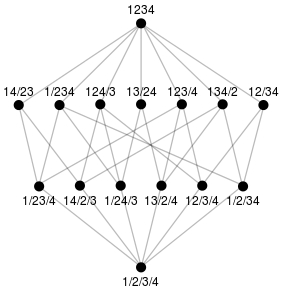
\includegraphics[scale=1]{Reticulo.jpg}   
	\caption{Retículo de subgrupos.}
	\label{Reticulo}
   \end{figure}

  \begin{theorem}[Teorema\IS de Lagrange]
   Si G es un grupo finito y H un subgrupo de G, entonces el número de elementos de H divide el número de elementos de G.
  \end{theorem}
  
  \begin{lemma}
   Sea $\varphi: G\rightarrow G$, son equivalentes:
   \begin{enumerate}
    \item $\varphi$  es inyectiva.
    \item $\varphi$  es biyectiva.
    \item $\varphi$  es sobreyectiva.
   \end{enumerate}
  \end{lemma}
  La demostración de este teorema es totalmente trivial. Con apoyarnos en que el conjunto G es finito, puede observarse que una de
  esas propiedades implica directamente las demas.
  
  \begin{lemma}
   Si $\varphi$  es un biyección y $A, B$ son subconjuntos de $G$:
   \begin{enumerate}
    \item $card(A)=card(\varphi(A))$
    \item $A=B \Leftrightarrow \varphi(A)=\varphi(B)$
    \item $\varphi(A\cap B)=\varphi(A)\cap\varphi(B)$
   \end{enumerate}
  \end{lemma}
  
  \begin{lemma}
   Sea $G$ un grupo finito, $g \in G\ y\ \varphi_{g}(x)=g*x$. Por la propiedad cancelativa, podemos ver que $\varphi_{g}$ es inyectiva.
   Además, por ser $G$ finito, sabemos que $\varphi_{g}$  es biyectiva.
  \end{lemma}
  También podemos definir $\varphi_{g}(H)=\{g*h\tq h\in H\}$
  \begin{lemma}
   $H<G\Rightarrow$  $H$ es subconjunto de $G$.
  \end{lemma}
  
  \begin{notacion}
   $gH=\varphi_{g}(H)$
  \end{notacion}

  \begin{corol} 
  Extraemos las siguientes conclusiones:
   \begin{enumerate}
    \item $g\in gH$
    \item $card(H)=card(gH)$
    \item $H=gH \Leftrightarrow  g \in H$
   \end{enumerate}
  \end{corol}

  \begin{proof}
   \begin{enumerate}
    \item $e \in  H$. Por tanto $g*e\in gH$. $g*e=g\in gH$.
    \item Se puede ver apoyándonos en los lemas anteriores puesto que $H$ es finito.
    \item $\Rightarrow: e \in H \Rightarrow e=gh$ con $h \in H \Rightarrow h=g^{-1}\in H \Rightarrow g \in H$.\\
	  $\Leftarrow: g \in H \Rightarrow g^{-1}\in H$ y todo elemento $h \in H$ cumple $h = g(g^{-1}h)\in H$.
   \end{enumerate}
  \end{proof}
  
  \begin{prop}
   Dados $g_{1}$,$g_{2}\in G$ y $H<G\Rightarrow g_{1}H=g_{2}H \vee g_{1}H\cap g_{2}H=\varnothing$
  \end{prop}
  \begin{proof}
   $g_{1}H\cap g_{2}H \neq \varnothing \Leftrightarrow$ $\exists h_{1},h_{2}$  t.q. $g_{1}h_{1}=g_{2}h_{2} \Rightarrow h_{1}=g_{1}^{-1}g_{2}h_{2} \Rightarrow h_{2}^{-1}h_{1}=g_{1}^{-1}g_{2}\in$H
   $\Leftrightarrow$ $g_{1}^{-1}g_{2}H=H \Rightarrow g_{2}H=g_{1}H$
  \end{proof}
  \begin{example}
   Tomando el famoso grupo $D_{4}$, podemos obtener $H=\{1,g,g²,g³\}$; $sH=\{s,sg,sg²,sg³\}$
  \end{example}
  
  \subsection{Particiones}
  \begin{defn}[Relación\IS de equivalencia]
   Fijado un conjunto $G\neq\varnothing$. Una relación R en G es de equivalencia si:
   \begin{enumerate}
    \item $\forall x\in G,  xRx$
    \item $\forall x,y \in G,  xRy \Leftrightarrow  yRx$
    \item $\forall x,y,z \in G,  xRy \wedge yRz \Rightarrow xRz$
   \end{enumerate}
  \end{defn}
  \begin{defn}[Partición]
   Familia de subconjuntos disjuntos dos a dos tales que su unión constituye el total.
  \end{defn}
  
  Una partición define una relación de equivalencia y viceversa. Si R es una relación de equivalencia en un grupo G, 
  definimos una partición en la que los subconjuntos son de la forma: $S_{x}=\{y\in G \tq xRy\}$
  
  \begin{proof}[Volvamos a demostrar la proposición 1.22]
   \\Definimos una relación de equivalencia R en G a partir del grupo H.
   $g_{1}Rg_{2} \Leftrightarrow g_{1}^{-1}g_{2}\in H$  y comprobamos que, efectivamente, esta relación es de equivalencia.
   Tenemos $S_{e}=H$. Así $S_{g}$  o ya cubre junto con H todo G, o cojo otro $g^{'}$  y repito el proceso con $S_{g^{'}}$.
   Así formare una serie de grupos de la forma $S_{x}$  disjuntos dos a dos y cuya unión me da G.\\
   De esta forma podemos ver que card(G)=card(H)*s
  \end{proof}
  
  \begin{corol}[Teorema de Lagrange]
   Dado g $\in$ G, siendo G un grupo finito $\Rightarrow$  ord(g) divide a |G| (cardinal de G). Así, suponiendo |G|=p primo,
   los únicos subrgupos que tiene G son los triviales: $<1>$ y  $G$
  \end{corol}
  \begin{theorem}
   Si |G|=p primo $\Rightarrow$  G es cíclico. Además, si |G|=n, $\forall$g ord(g) divide a n $\Rightarrow$  $g^{n}=e$
  \end{theorem}
  \begin{example}
   Con ayuda de este teorema puede demostrarse el pequeño teorema de Fermat. 
   Definimos $\mathbb{Z}/p\mathbb{Z}=\{\bar{0},\bar{1}...,\bar{p-1}\}$.
   Si tomamos el grupo de las unidades de $\mathbb{Z}/p\mathbb{Z}$ tenemos $\{\bar{1}, \bar{2},....\bar{p-1}\}$ $\Rightarrow$
   $\bar{a}\in\mathbb{Z}/p\mathbb{Z} \wedge \bar{a}\neq 0 \Rightarrow a^{p-1}=\bar{1}$.
  \end{example}
  \begin{theorem}
   Si |G|=$p^{2}$  con p primo $\Rightarrow$  $\exists g \in G \tq ord(g)=p$
  \end{theorem}
  \begin{proof}
   Tomamos $g \in G \wedge g\neq e \Rightarrow ord(g)=p$  ó $ord(g)=p^{2}$. En el primer caso ya lo tenemos, vamos a por el segundo.
   $ord(g)=p^{2}\Rightarrow ord(g^{p})=p$
  \end{proof}
  \begin{example}
   Por todo lo explicado anteriormente, si tomamos el anillo de polinomios $\mathbb{Z}/p\mathbb{Z}[x]$, tenemos $X^{p-1}-\bar{1}=
   \prod_{\bar{a}\in\mathbb{Z}/p\mathbb{Z} \wedge \bar{a}\neq 0}(x-\bar{a})$
  \end{example}
  
  \begin{theorem}[Teorema\IS de Lagrange, otra visión]
   Dados $H<G$  $\exists a_{1},...,a_{r}\in G\tq$  G=$a_{1}H \cup a_{2}H.... \cup a_{r}H$  $\wedge a_{i}H\cup_{j}H=\varnothing \forall i,j$.
   Es decir, $|G|=r|H|$
  \end{theorem}

  Definimos ahora otra relación a partir de $H<G$: $cR^{'}d \Leftrightarrow cd^{-1}\in H$. La comprobación de que esto es una relación
  la omitiremos por ser trivial. En esta parItción, el conjunto de elementos relacionados con d es: $Hd=\{hd/h\in H\}$
  \begin{defn}[Subgrupo\IS normal]
   Decimos que $H<G$  es un subgrupo normal si aH=Ha $\forall$a. Por tanto, si G es un grupo abeliano, H también lo será y cualquier
   subgrupo será normal. Un subgrupo normal se expresa como $H\lhd G$
  \end{defn}
  \begin{example}
   Tomamos G=$\mathbb{Z}$  y H=$4\mathbb{Z}$. 
   El subgrupo de los elementos que son equivalentes a n es nH=$\{n*4k\tq k \in \mathbb{Z}\}$.
   En este caso tenemos 4 subgrupos según esta condición: $\bar{0},\bar{1},\bar{2},\bar{3}$
  \end{example}
  
  Si $H\lhd G$  podemos definir una estructura de grupo en el subconjunto de clases, lo que se llamará el grupo cociente.
  
  \begin{defn}[Grupo\IS cociente] Sea $H \lhd G$. Definimos $G / H$ como el conjunto de todas las clases laterales izquierdas, es decir
  
  \[ G/H = \{ aH \tq a \in G\} \]
 \end{defn}
  
  
  Dados $g_{1}H$  y $g_{2}H$  podemos formar el conjunto $\{h_{1}\ast h_{2}\tq h_{1}\in g_{1}H \wedge h_{2}\in g_{2}H\}$. Si operamos   $g_{1}H\ast g_{2}H=(g_{1}\ast g_{2})H$  que es otra clase. Por tanto el grupo de clases es cerrado.
  
  El neutro sería la caja $H$ puesto que $gHH=gH$ para cualquier $g$ que escojamos. Además el inverso de $gH$ es $g^{-1}H$.
  
  Por último, vemos que $(g_{1}H\ast g_{2}H)\ast g_{3}H=g_{1}H\ast Hg_{2}\ast g_{3}H=g_{1}H\ast Hg_{3}\ast g_{2}H$, por ser G asociativo. Queda probado pues, que el conjunto de las clases de equivalencia, forma un grupo.
  
\begin{defn}[Índice\IS de un subgrupo] El índice de un subgrupo $H$ de $G$ es el \textit{tamaño relativo} de $H$ en $G$, el número de \textit{copias} de $H$ que llenarían $G$.  

Estrictamente, se define $[G:H]$ es el número de clases laterales de $H$ en $G$. Si $H$ y $G$ son finitos, entonces 

\[ [G:H] = \frac{\card{G}}{\card{H}} \]
\end{defn}

  \begin{theorem}
   Si definimos [G:H]=nº de cajas=índice, tenemos:
   H$<$G $\wedge[G:H]=2 \Rightarrow H \lhd G$.
  \end{theorem}
  \begin{proof}
   Por un lado tenemos que g$\notin$H $\Rightarrow$  gH= $H^{c}$.
   Por otro lado, si tomamos la otra relación de equivalencia, a partir de g$\notin$H obtenemos Hg=$H^{c}$.
   Uniendo estos dos ejemplos, donde mantenemos H como una mitad en ambos, tenemos Hg=gH. Por tanto H es un subgrupo normal
  \end{proof}
  
  \begin{lemma}
   Dadas dos particiones formadas por los subconjuntos $aH$ y $Ha$ para un elemento $a \in G$ y con $H <G$, podemos definir dos aplicaciones $\pi$ y $\pi '$ que lleven cada elemento de G a su respectiva caja:
   $$\appl{\pi}{G}{G/H}$$
   $$\appl{\pi'}{G}{G/H}$$
   Tenemos entonces que:
   $$H \text{subgrupo normal} \implies \text{la partición izquierda coincide con la derecha}\ (a_iH = Ha_i)$$
   $$H \text{subgrupo normal} \implies \pi \ =\ \pi '$$

   
   Además, si H es normal
   \begin{enumerate}
	\item Podemos definir una operación en el conjunto cociente.     
	\item $\appl{\pi}{G}{G/H}$ es compatible con las operaciones.
   \end{enumerate}
  \end{lemma}
  
  \begin{example}
	Sea $Q$ el grupo formado por las raíces cuartas de 1.\\
	$$Q = \{ 1, i, j, k, -1, -i, -j, -k\} $$\\
	Podemos ver que $Q$ se genera a partir de los elementos $i, j, k$.\\
	$$Q = <i,j,k>$$\\
	Además vemos que $-1$ conmuta con todos los elementos del grupo: $-1 \in Z(G)$
	Analizamos el retículo del grupo y vemos que esta formado por los subgrupos:
	\\
	$Orden\ 1 = \{ 1\} $\\
	$Orden\ 2 = \{ 1, -1\} $\\
	$Orden\ 4 = \{ 1, i, i^2, i^3\},\
			  \{ 1, j, j^2, j^3 \},\
			  \{ 1, k, k^2, k^3 \}.$\\
		  
	El grupo no es abeliano, sin embargo, todos sus subgrupos son normales porque todo subgrupo $H<G$ de indice 2 (es decir, el conjunto de clases $G/H$ tiene dos elementos) es normal.
	
  \end{example}
  
    \begin{defn}[Centro]
	Llamamos centro del grupo $G$ al grupo formado por todos los elementos que conmutan con todos los elementos de $G$.:\\
	$$Z(G) = \{ a\in G\tq a\ast g = g\ast a\ \forall g\in G\} $$
	Además, tenemos que:
	$aZ(G)=Z(G)a \implies Z(G)\lhd G$
  \end{defn}
   
 Dados un grupo G y un subconjunto no vacío S, defino $S^{-1}=\{s^{-1}\tq s\in S\}$. Dados $S_{1},S_{2}<G$, defino  \[ (S_{1}\ast S_{2})^{-1}=\{s_{1}\ast s_{2}\tq s_{1}\in S_{1} \wedge s_{2}\in S_{2}\} \]
 
 que operando, nos queda que 
 
 \begin{align*}
 (S_1 \ast S_2)^{-1} &= \{s_{1}^{-1}\ast s_{2}^{-1}\tq s_{1}\in S_{1} \wedge s_{2}\in S_{2}\}\\
 &= \{s_{1}^{-1}\ast s_{2}^{-1}\tq s_{1}^{-1}\in S_{1}^{-1} \wedge s_{2}^{-1}\in S_{2}^{-1}\} \\
 & =S_{2}^{-1}\ast S_{1}^{-1}
 \end{align*}
 
 Sea H un subgrupo de G, entonces $H^{-1}=H$.
 
 \begin{theorem}
  Fijado un grupo G y $H_{1}, H_{2}$  subgrupos de G entonces: $H_{1} \lhd G \implies H_{1}\ast H_{2}<G$. 
 \end{theorem}
 
 \begin{proof}
  Sabemos que $H_{1}\ast H_{2}=H_{2}\ast H_{1}$. Para ver que $H_{1}\ast H_{2}<G$  hay que comprobar que está
  \begin{enumerate}
   \item Cerrado por la operación: $(H_{1}\ast H_{2})\ast (H_{2}\ast H_{1})=H_{1}\ast (H_{2}\ast H_{2})\ast H_{1}=H_{1}\ast H_{1}\ast H_{2}\ast H_{2}=H_{1}\ast H_{2}$
   \item Todo elemento tiene inverso, es decir: $\alpha\in H_{1}\ast H_{2}\Rightarrow \alpha^{-1}\in H_{1}\ast H_{2}$. Pero entonces tenemos:
   $\alpha^{-1}\in (H_{1}\ast H_{2})^{-1} = H_{2}^{-1}\ast H_{1}^{-1}=H_{2}\ast H_{1}=H_{1}\ast H_{2}$ que también contiene a $\alpha$ \textit{por ejemplo.}
  \end{enumerate}
 \end{proof}

 \begin{example}
  Tomamos el ya famoso grupo $D_{4}=\{1,g,g^{2},g^{3}, s, sg, sg^{2}, sg^{3}\}=\gen{s,g}$.
  
  Dentro de este grupo, el elemento 1 tiene orden dos, los elementos $g$, $g^{3}$  tienen orden 4 y el resto, 2.
  \begin{gather*}
  Z(D_{4})= \{\alpha\in D_{4} \tq \alpha\beta=\beta\alpha \ \forall \beta \in D_{4}\}= \\
  = \{\alpha\in D_{4}\tq \alpha s = s\alpha \wedge \alpha g = g\alpha\}=\{1, g^{2}\}=\gen{g^{2}}
  \end{gather*} 
  
  Este subgrupo es normal.
  
  Para contruir el retículo de subgrupos tomamos, en primer lugar, el único grupo de un elemento: 
  \[ \{1\} \]
  Ahora tomamos los grupos de orden dos, que serán todos aquellos generados por elementos que tienen orden dos:\\
  \[ \gen{sg^{3}}, \gen{sg}, \gen{g^{2}}, \gen{s}, \gen{sg^{2}} \]
  
  Los subgrupos de orden cuatro son los formados por elementos de orden 4 más los obtenidos al combinar el centro con los demás subgrupos de orden 2:
  \[ \{1,g,g^{2},g^{3}\}, \ \gen{g}, \ \{1, g^{2}, s, sg^{2}\} \]
 \end{example}
 

 \begin{proof}
 \begin{enumerate}
  \item $\Rightarrow$  Obvio, tan obvio como que $D_4$ le apasiona al profesor.
  \item $\Leftarrow$\\
  $aHa^{-1} \subset H \ \Rightarrow \ a^{-1}Ha\subset H.$. Por tanto $a^{-1}aHa^{-1}a \subset a^{-1}Ha \ \Rightarrow \ a^{-1}Ha \subset  a^{-1}Ha \Rightarrow \ H \subset a^{-1}Ha$.
  Contención a derecha e izquierda implica igualdad.
 \end{enumerate}
 \end{proof} 
 
 \subsection{Homomorfismos de grupos}
 \begin{defn}[Homomorfismo]
 Sea f $\appl{f}{(G_1, \cdot )}{(G_2, \ast )}$. $f$ es un homomorfismo de grupos si 
 \[ f(a\cdot b) = f(a)\ast f(b) \]
\end{defn}
 
 \begin{example}
 Si consideramos la aplicación $\appl{\pi}{G}{G/N}$ que lleva los elementos de $G$ a su respectivo conjunto cociente, la función sobreyectiva $\pi$ es un homomorfismo de grupos si $N\lhd G$.
 \end{example}
 
 \begin{props} 
 Si $\appl{f}{G_1}{G_2}$ es un homomorfismo de grupos, entonces
 \begin{enumerate}
 \item $f(e_1) = e_2$ con $e_1$ neutro de $G_1$ y $e_2$ neutro de $G_2$
 \item $f(x^{-1}) = f(x)^{-1}$
 \end{enumerate}
 \end{props}
 
 \begin{proof} \\
 
 1) \begin{align*}  
 e_1\cdot e_1 &= e_1 \\
 f(e_1)& =f(e_1\cdot e_1) = f(e_1)\ast f(e_1) \\
 f(e_1) &= e_2 \ast e_2 = e_2
 \end{align*}

 2) \begin{align*}
 f(x\cdot x^{-1}) &= f(e_1) = e_2 \\ 
 f(x)\ast f(x^{-1}) &= e_2 \\
  f(x^{-1}) &= f(x)^{-1}
  \end{align*}
 
 \end{proof}
 

\begin{remark} Si $G$ es un grupo finito \[\ord{f(a)}\ |\;\ord{a}\, \forall a \in G_1 \] \end{remark}

\begin{lemma}
La composición de dos homomorfismos de grupos es un homomorfismo de grupos.
\end{lemma}

\begin{defn}[Núcleo\IS de un homomorfismo]
Dado $\appl{f}{G_1}{G_2}$ el núcleo de $f$ se define como 
\[ \ncl{f} = \{ a\in G_1 \tq f(a) = e_2\} \]
con $e_2$ el elemento neutro de $G_2$. 

Además, se cumple que $\ncl f = \{ e_1 \}$ si y sólo si $f$ es inyectiva.
\end{defn}

\begin{theorem}
 Sea $\appl{f}{G_1}{G_2}$ un homomorfismo de grupo. Entonces $\ncl f$ y $\img f$ son subgrupos de $G_1$ y $G_2$ respectivamente, con $\ncl f$ el núcleo de la aplicación y $\img f$ la imagen de la misma.
 \end{theorem}
 
 \begin{proof} Empezamos demostrando que el núcleo es un subgrupo.
 \begin{gather*}
  \ncl f < G_1 \\
 e_1 \in \ncl f \\
 x, y \in \ncl f \implies xy^{-1}\in \ncl f \\
 f(xy^{-1}) = \underbrace{f(x)}_{e_2} \underbrace{f(y)^{-1}}_{e_2^{-1}} = e_2
 \end{gather*}
 
Pasamos ahora a demostrarlo con la imagen.

\begin{gather*}
\img f < G_2 \\
 e_2\in \img f \implies e_2 = f(e_1)\\
 a\in \img f \implies a^{-1}\in \img f\\
 \exists \alpha \in G_1 \tq a=f(\alpha ) \implies a^{-1} = (f(\alpha ))^{-1} = f(\alpha ^{-1})
 \end{gather*}
 
 \end{proof}

\begin{defn}[Epimorfismo]
Sea $\appl{f}{G_1}{G_2}$ un homomorfismo de grupos. Entonces diremos que $f$ es un epimorfismo si $\img f = G_2$.
\end{defn}

\begin{defn}[Monomorfismo]
Sea $\appl{f}{G_1}{G_2}$ un homomorfismo de grupos. Entonces diremos que $f$ es un monomorfismo si $\ncl f = \{ e_1\} $
\end{defn}

\begin{lemma} Sea $\appl{f}{G_1}{G_2}$ un homomorfismo de grupos, entonces se tiene que

\[ \ncl f \lhd G_1 \]
\end{lemma}

\begin{proof} Recordemos la definición de subgrupo normal:
\[ H \lhd G_1 \dimplies \forall a\in G_1\ aHa^{-1}\subset H \]
En este caso, tenemos que
\[ \forall a\in G_1\ a\ncl{f}a^{-1} = \{aha^{-1} \tq h\in \ncl{f} \} \]

Si tomamos $f\left(a\ncl{f}\inv{a}\right)$, vemos que es igual a \[ f(a) f(\ncl{f}) f(\inv{a}) = \alpha e_2 \inv{\alpha} = e_2 \]
\end{proof}

\begin{remark}El único homomorfismo de $\ent/n\ent$  en $\ent$, y en general de un grupo finito a los enteros, es el trivial. Esto se debe
a que dado $a\in\ent/n\ent$, ord(a)=$\alpha$, pero $\ord{f(a)}$ será infinito, salvo que $f(a)=0$.\end{remark}
  
\begin{lemma} Si $N\lhd G$ entonces $G/N$ tiene estructura de grupo y $\appl{\pi}{G}{G/N}$  (homomorfismo que manda cada
elemento a su grupo cociente)  es un epimorfismo.
\end{lemma}

\begin{corol}
 Dado $\appl{f}{G_1}{G_2}$  un homomorfismo de grupos, ya vimos que si f era un monomorfismo (inyectivo) en N(f)=$\{e_1\}$. \\
 Esto se debe
 a que hago que dentro de aN, sólo este a, ya que en caso contario, tomando b$\in$N, por lo explicado anteriormente, llegaríamos
 a f(a)=f(b), por lo que la función ya no sería inyectiva.
\end{corol}

\begin{defn}[Isomorfismo]
Diremos que f es un isomorfismo si existe un homomorfismo de grupo $\appl{g}{G_2}{G_1}$  de tal forma que f$\circ$g=id. El hecho de
que f sea isomorfo, implica, por definición, que f es un homomorfismo y que es biyectivo.
\end{defn}

Partiendo de $\appl{f}{G_1}{G_2}$  un homomorfismo de grupos, se cumple que:
\begin{enumerate}
 \item $H<G_1 \ \Rightarrow \ f(H)<G_2$
 \item $H_2<G_2 \ \Rightarrow \ f^{-1}(H_2)<G_1$
 \item $H_2 \vartriangleleft G_2 \ \Rightarrow \ f^{-1}(H_2)\vartriangleleft G_2$
 \item f sobreyectiva y $H_1 \vartriangleleft G_1 \ \Rightarrow \ f(H_1)\vartriangleleft G_2$
\end{enumerate}
\begin{proof}
Recordamos que dado S un suconjunto de G, para probar que S es un subgrupo bastaba con ver que $S \neq \varnothing$  y que $xy\in S \ \Rightarrow \ y^{-1}x\in S $
 \begin{enumerate}
  \item f(H) $\neq \varnothing$\\
  $a,b\in f(H) \tq a=f(x) y b=f(y) \Rightarrow \ b^{-1}a=f^{-1}(y)*f(x)=f(y^{-1}x)\in H$
  \item $f^{-1}(H)\neq \varnothing$\\
  $f(x)=a, f(y)=b \Rightarrow \ xy\in f^{-1}(H_2) \Rightarrow \ y^{-1}x=f(y^{-1}x)\in f^{-1}(H_2)$
  \item Si tomo $\appl{\varphi}{G_2}{G_2/H_2}$  un homomorfismo de grupos. Dado que la composición de homomorfismos es otro homomorfismo, 
  tenemos que $\varphi \circ f$  es un homomorfismo. Además, el núcle de $\varphi$  es $H_2$, por lo que el núcleo de la composición sera $f^{-1}(H_1)$.
  Por otro lado, ya hemos visto que el núcleo de un homomorfismo es un subgrupo normal del grupo de partida. Por tanto $f^{-1}(H_1) \vartriangleleft G_1$
 \end{enumerate}
 \end{proof}

\begin{defn}[Isomorfismo]
Un homomorfismo de grupos $\appl{f}{G_1}{G_2}$ es un isoformismo si existe un homomorfismo de grupos $\appl{g}{G_2}{G_1}$ tal que $g\circ f = id_{G_1}$ y $f\circ g = id_{G_2}$. 
\end{defn}


\begin{remark} Dados dos grupos $G_1$ y $G_2$, $\appl{f}{G_1}{G_2}$ es un isomorfismo de grupos si y sólo si f es un homomorfismo y es una biyección de conjuntos.
\end{remark}

\begin{lemma}
Sea $\appl{f}{G_1}{G_2}$, entonces:
\begin{enumerate}
\item Si $H_1$ es un subgrupo de $G_1$, $f(H_1)<G_2$
\item Si $H_2 < G_2$, entonces $f^{-1}(H_2)<G_1$
\item Si $H_2 \lhd G_2$, $f^{-1}(H_2)\lhd G_1$
\item Si $f$ es sobreyectiva y $H_1\lhd G_1$, tenemos que $f(H_1)\lhd G_2$
\end{enumerate}
\end{lemma}

\begin{proof}
\paragraph{Propiedad 1}
\begin{gather*}
e_2 \in f(H_1)\\
x, y\in f(H_1) \implies xy^{-1}\in f(H_1)\\
x=f(a);\; y = f(b);\; a, b\in H_1\\
xy^{-1}=f(a)f(b)^{-1} = \underbrace{f(ab^{-1})}_{H_1} \in f(H_1)
\end{gather*}

\paragraph{Propiedad 2}
\begin{gather*}
e_1 \in f^{-1}(H_2)\\
a, b \in f^{-1}(H_2) \implies ab^{-1} \in f^{-1}(H_2)\\
f(a) \in H_2;\; f(b) \in H_2 \implies \underbrace{f(ab^{-1})}_{f(a)f(b)^{-1}}\in H_2
\end{gather*}

\paragraph{Propiedad 3}
$f^{-1}(H_2) = N(\pi \circ f)$. Como $f^{-1}(H_2)$ es el núcleo de h de g entonces $f^{-1}(H_2)\lhd G_1$.
\end{proof}


Sea $\appl{f}{G_1}{G_2}$ un homomorfismo de grupos, y $f$ sobreyectiva (es decir, un \textit{epimorfismo})
vamos a analizar el retículo de subgrupos de $G_2$.\\
Fijado un subgrupo $H_2<G_2$ le asociamos un subgrupo $f(H_2)<G_1$. Asociamos al retículo de subgrupos de $G_2$ subgrupos de $G_1$ que contienen al núcleo $N(f)$.
\begin{theorem}
Es posible identificar el retículo de subgrupos de $G_2$ con los subgrupos de $G_1$ que contienen al núcleo $N(f)$
\end{theorem}

\obs Sea $\appl{f}{G_1}{G_2}$ sobreyectiva. $H$ subgrupo de $G_1$ que contiene al núcleo $N(f)$. Entonces $H = f^{-1}(f(H))$
Como $f(H)$ es un subgrupo de $G_2$ la observación indica que todo subgrupo de $G_1$ que contiene al núcleo es de la forma $f^{-1}(K)$ para algún subgrupo K de $G_2$

\begin{example}
El retículo de subgrupos de $Q/{\{ -1, 1 \} }$ se identifica con los subgrupos de $Q$\footnote{Grupo de cuaterniones, osea, raíces cuartas de uno.} que contienen al núcleo $\{ 1, -1\} $.
\end{example}

\begin{defn}[Grupos\IS isomorfos]
Dos grupos son isomorfos si existe un isomorfismo entre ellos.
\end{defn}

\begin{theorem}
Si $\appl{f}{G_1}{G_2}$ es un homomorfismo de grupos entonces $Img(f)$ (subgrupo de $G_2$) es isomorfo al grupo cociente $G_1/{N(f)}$\footnote{Recordad que $\ncl f \lhd G_1$}
\end{theorem}

\begin{example}
Si tenemos la aplicación 
\begin{gather*}
\appl{h}{\mathbb{Z}}{\mathbb{C}^*}\\
1 \longrightarrow i\\
k\longrightarrow ik\\
\end{gather*}

$\ncl f = 4\mathbb{Z} < \mathbb{Z}$\\
$Img(f) = \{1, i, -1, -i \}$
Tenemos que $\{ 1, i, -1, -i \}$ es isomorfo al grupo $(\mathbb{Z} /4\mathbb{Z}, +)$
\end{example}

\newpage
\printindex
\end{document}
